\documentclass{article}
\usepackage[utf8]{inputenc}
\usepackage[english]{babel}
\usepackage[]{amsthm}
\usepackage[]{amssymb}
\usepackage[]{amsmath}
\usepackage{graphicx}
\usepackage{listings}
\usepackage{pdfpages}
\lstset{language=Matlab}

\title{SP21 COMPSCI 513 - Homework 5}
\author{Zijie Zhang}
\date\today

\begin{document}
\maketitle
\section*{Q1}
All the necessary calculation details are in the next four pages.
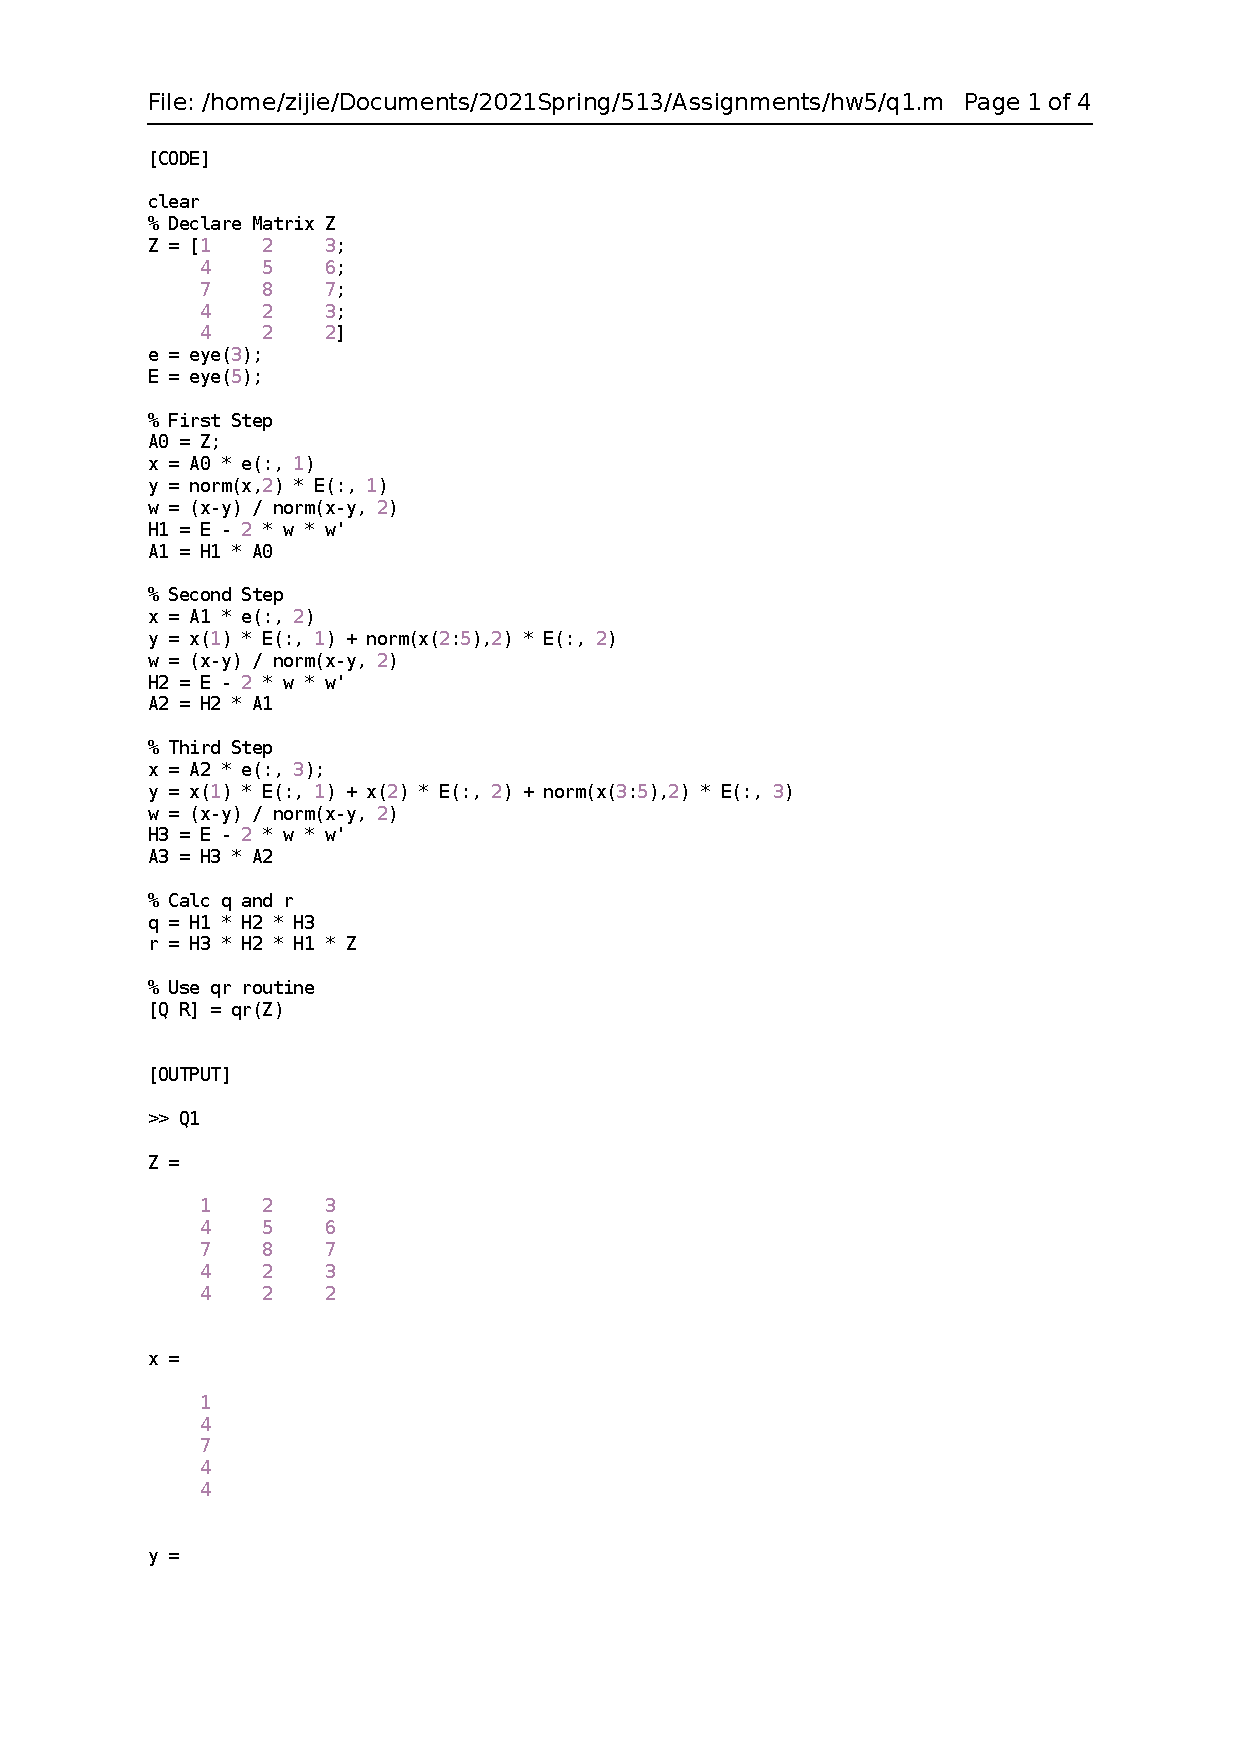
\includepdf[pages=-]{Q1_sol.pdf}
\section*{Q2}
\begin{itemize}
    \item[(a)] Take a look at the structure of the $H$ matrix.
                    $$H = I - 2ww'$$
                When compute $Hv$, we have $$Hv = (I - 2ww')v = v - 2 ww'v$$
                Here, the computational complexity of $w'v$ is $O(m)$, the computational complexity of $v - 2w(w'v)$ is $O(m)$. So the final computational complexity is still $O(m)$.\\
                In conclusion, this algorithm is more efficient.
    \item[(b)] [CODE] fast\_qr.m\\
                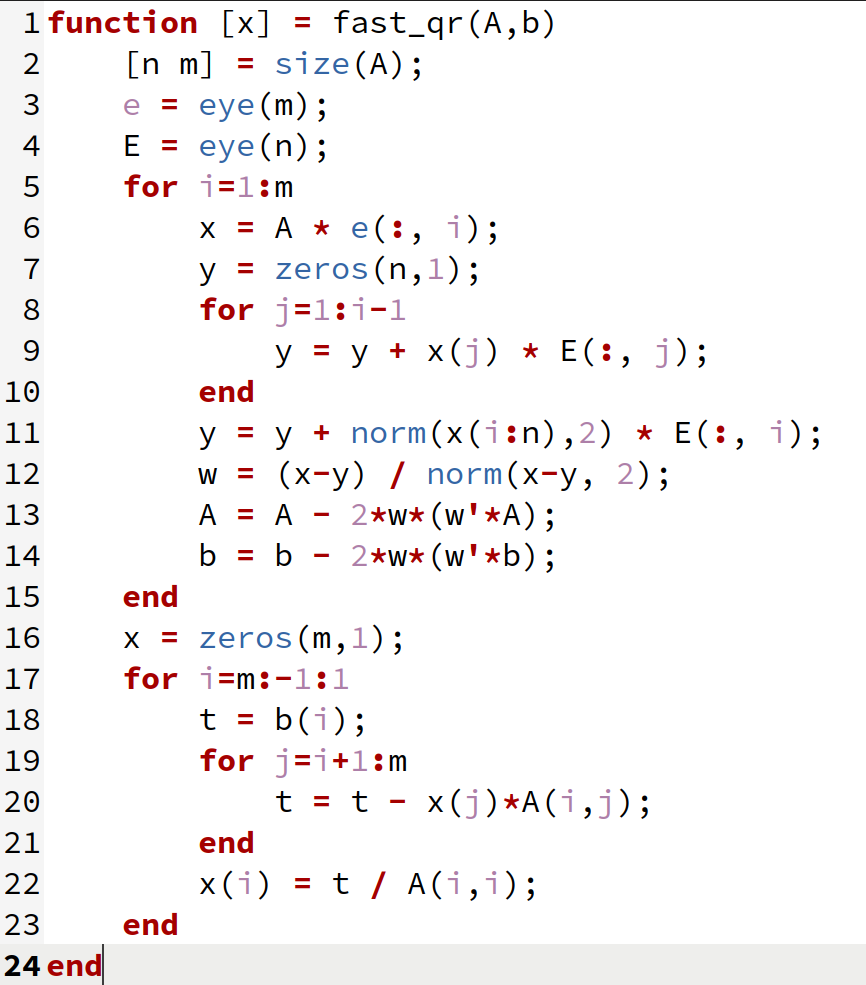
\includegraphics[width=12cm]{fast_qr.png}
    \item[(c)] Run examples:\\
                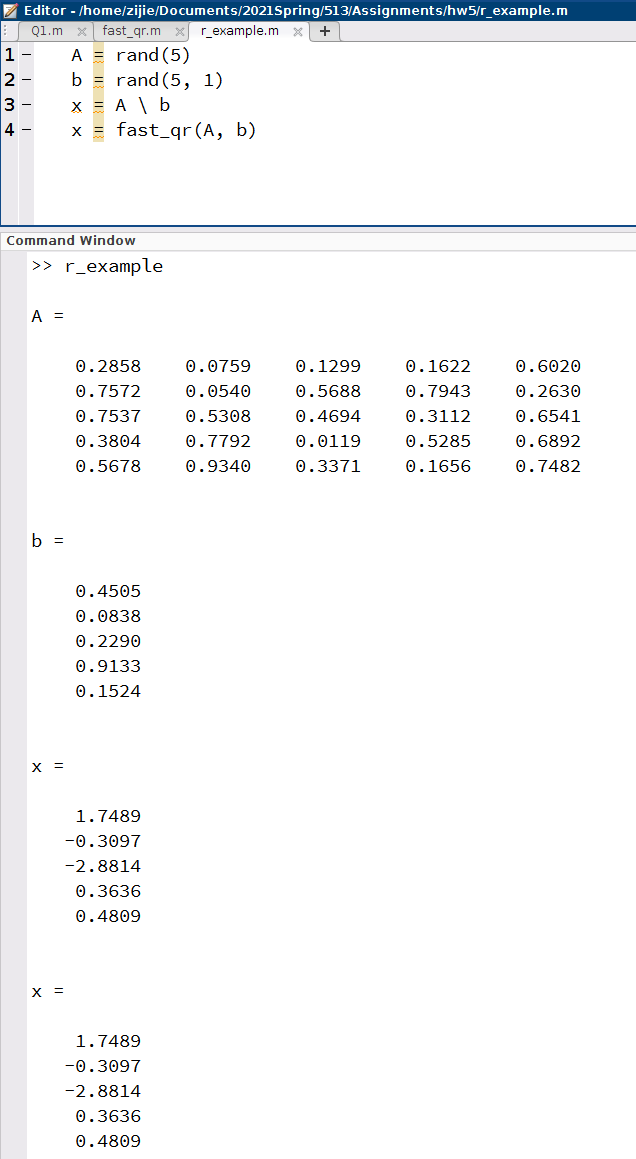
\includegraphics[width=6cm]{ex1.png}
                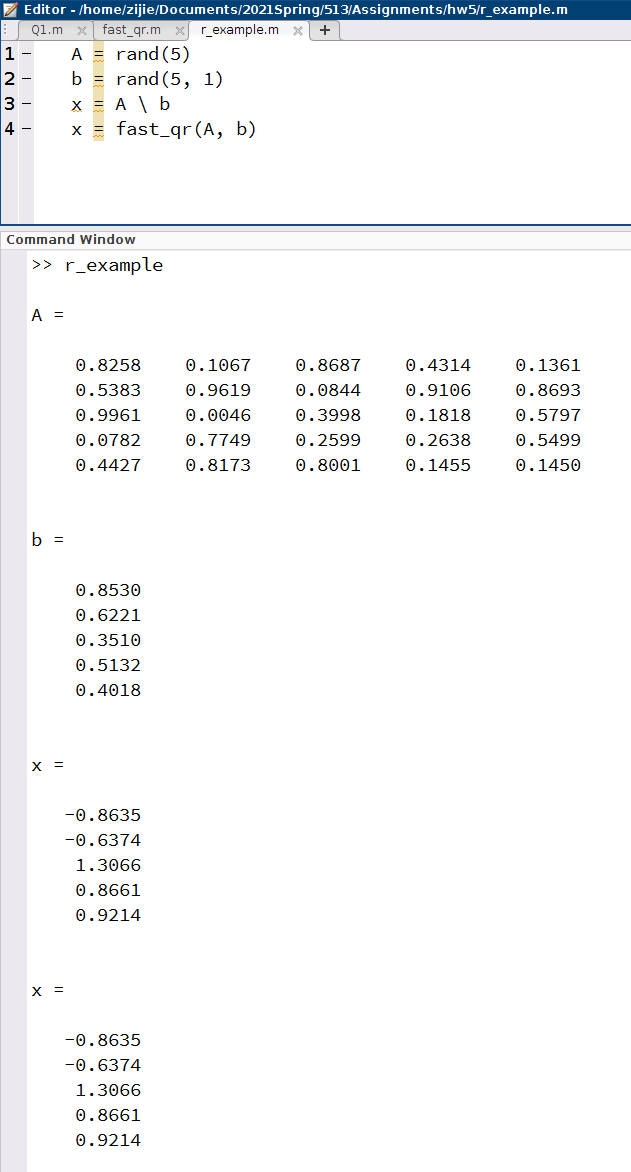
\includegraphics[width=6cm]{ex2.png}
    \item[(d)]
                Take a look at the code above.\\
                Suppose $A$ is $n \times m$.\\
                Calculate $x, y, w$ cost $O(n)$\\
                Calculate new $A$ cost $O(mn)$\\
                Calculate new $b$ cost $O(m)$\\
                With $m$ times iteration, the total calculation complexity is $O(m^2n)$.

\end{itemize}
\end{document}